\documentclass[conference]{IEEEtran}
\usepackage{blindtext, graphicx}
%\usepackage{cite}
% \cite{} output to follow that of IEEE. Loading the cite package will
% result in citation numbers being automatically sorted and properly
% "compressed/ranged". e.g., [1], [9], [2], [7], [5], [6] 
\usepackage[cmex10]{amsmath}

\usepackage[backend=biber]{biblatex}
\addbibresource{ref.bib}

% correct bad hyphenation here
%\hyphenation{op-tical net-works semi-conduc-tor}

\begin{document}
%
% paper title
% can use linebreaks \\ within to get better formatting as desired
\title{Predicting Hospital Readmission Rate of Diabetic Patients}


% author names and affiliations
% use a multiple column layout for up to three different
% affiliations
\author{\IEEEauthorblockN{Ashish Kumar}
\IEEEauthorblockA{Department of Mining Engineering\\
McGill University\\
ashish.kumar@mail.mcgill.ca}
\and
\IEEEauthorblockN{Charlie Bloomfield}
\IEEEauthorblockA{School of Computer Science\\
McGill University\\
charles.bloomfield@mail.mcgill.ca}
\and
\IEEEauthorblockN{Jonathan Campbell}
\IEEEauthorblockA{School of Computer Science\\
McGill University\\
jonathan.campbell@mcgill.ca}}

% make the title area
\maketitle

%\boldmath

\begin{abstract}

Using an existing dataset of patient-hospital encounters, we present methodology for predicting the readmission of diabetic patients based on selected features of the encounters. An existing dataset of encounters from 130 U.S. hospitals was used~\cite{dataset-2014} and pre-processing of this dataset is discussed with respect to problems of class imbalances and missing data. The best performance was obtained using Support Vector Machines with a precision value of 61\%.

\end{abstract}

% An example of a floating figure using the graphicx package.
%\begin{figure}[!t]
%\centering
%\includegraphics[width=2.5in]{myfigure}
% where an .eps filename suffix will be assumed under latex, 
% and a .pdf suffix will be assumed for pdflatex; or what has been declared
% via \DeclareGraphicsExtensions.
%\caption{Simulation Results}
%\label{fig_sim}
%\end{figure}

% An example of a double column floating figure using two subfigures.
% (The subfig.sty package must be loaded for this to work.)
% The subfigure \label commands are set within each subfloat command, the
% \label for the overall figure must come after \caption.
% \hfil must be used as a separator to get equal spacing.
% The subfigure.sty package works much the same way, except \subfigure is
% used instead of \subfloat.
%
%\begin{figure*}[!t]
%\centerline{\subfloat[Case I]\includegraphics[width=2.5in]{subfigcase1}%
%\label{fig_first_case}}
%\hfil
%\subfloat[Case II]{\includegraphics[width=2.5in]{subfigcase2}%
%\label{fig_second_case}}}
%\caption{Simulation results}
%\label{fig_sim}
%\end{figure*}

% An example of a floating table. Note that, for IEEE style tables, the 
% \caption command should come BEFORE the table. Table text will default to
% \footnotesize as IEEE normally uses this smaller font for tables.
% The \label must come after \caption as always.
%
%\begin{table}[!t]
%% increase table row spacing, adjust to taste
%\renewcommand{\arraystretch}{1.3}
% if using array.sty, it might be a good idea to tweak the value of
% \extrarowheight as needed to properly center the text within the cells
%\caption{An Example of a Table}
%\label{table_example}
%\centering
%% Some packages, such as MDW tools, offer better commands for making tables
%% than the plain LaTeX2e tabular which is used here.
%\begin{tabular}{|c||c|}
%\hline
%One & Two\\
%\hline
%Three & Four\\
%\hline
%\end{tabular}
%\end{table}

\section{Introduction}

Diabetes affects 336 million people worldwide and is predicted to increase to 552 million in 2030~\cite{estimates-2011}. Prediction of relevant factors resulting in readmission of diabetic patients is very important to reduce the large physical and finanical costs associated with readmission. This paper deals with the prediction of readmission of diabetic patients using a machine learning approach on a pre-existing dataset. We describe related research with said dataset in section 2, followed by a brief description of the dataset in section 3. Due to particularities with the dataset, several data pre-processing methods were performed and are discussed in section 4, followed by an explanation of the performance measurement criteria used in the project in section 5. We continue with brief descriptions of machine learning algorithms used, including baseline methods, with some focus on methods known to perform better on the dataset. The paper concludes with presentation and discussion of results and future work.

\subsection{Target Prediction Task}

As said above, the goal of this paper is to predict the readmission of diabetic patients based on various features recorded during their hospital visits. There are three target classes: readmitted before 30 days (class 1), after 30 days (class 2), or not readmitted at all (class 3).

\section{Related Work}

Diabetes or “diabetes mellitus” is a metabolic disorder characterized by hyperglycemia and disturbance of metabolism of fat protein and carbohydrates, caused by imperfections of insulin secretion or functioning~\cite{worldhealthorganization-2015}. Morbidity of patients in hospitals is significantly determined by the management of hyperglycemia in the hospitalized patients~\cite{hyperglycemia-2002, unrecognizeddiabetes-1998}. Readmission of patients to hospitals impacts the economy and quality of healthcare services. In terms of cost, readmission of patients cost the United States \$41.3 billion in 2011~\cite{estimates-2011}, out of which unchecked diabetes accounted for 23,700 readmissions at a cost of \$251 million~\cite{sas-2015}. Rising readmission rates have prompted the Centers for Medicare \& Medicaid Services (CMS) to introduce measures to curb the problem~\cite{readmissionreduction-2015}.

The impact of HbA1c measurement on hospital readmission rates was studied with the same dataset we are using using a multivariate logistic regression algorithm~\cite{hba1c-2014}. Although the research showed the importance of this feature, a study of other relevant features was excluded. Another paper used a commercial Support Vector Machine algorithm (SAS Enterprise Miner) on the same dataset and obtained an accuracy of 63.7\%~\cite{sas-2015}, but the handling of missing data was not properly managed and medical speciality of the attending doctor was removed, which is an important feature in deciding the outcome of the medical services rendered and eventually the readmission prediction. Furthermore, the measurement criteria used was the mis-classification rate, which is unreliable due to the imbalance of target classes. The demographics of diabetic patients were predicted using the same database in another paper on the same dataset~\cite{cotha-2015}, and the authors obtained an accuracy of 53.3\% using an ensemble method of decision trees.

\section{Dataset Description \& Analysis}

% discuss presence of missing data, what the features are, amount, where dataset came from...

\begin{figure}[htpb]
	\centering
	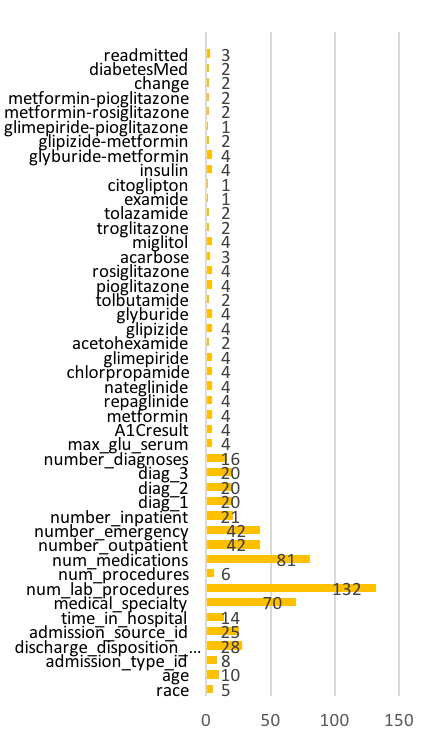
\includegraphics[width=0.4\textwidth]{dataset}
	\caption{Number of unique values for each feature in the dataset.}
	\label{fig:dataset}
\end{figure}

A ten-year clinical database of 130 U.S. hospitals was used for our target prediction task~\cite{dataset-2014, hba1c-2014}. The dataset has 101,766 instances with 49 features (demographics, diagnoses, hbA1c measurement, etc.) with one target feature. The features are categorical and continuous and were encoded as described in the appendix for the application of machine learning algorithms. The number of possible values after encoding for each features is mentioned in Figure~\ref{fig:dataset}.

Duplicate encounters of patients were removed from the database to satisfy the I.I.D (Independent and Identically Distributed) assumption of the classification algorithms. Class imbalance and problems of missing data are described and dealt in Sections 4.2 and 4.3 respectively.

\section{Data Pre-processing}

% discuss categorization of data
% smote, over sampling

Medical database especially diabetic database is associated with lot of anomalies. Pre-processing of the database is first and foremost step before proceeding further with the machine learning approaches.

\subsection{Feature Selection}
% removal of certain features not relevant (as per paper), possible combination of target into 2 classes...
Feature selection is a technique that reduces the dimension of a dataset's feature space. With high-dimensional data, especially when the dimension of a feature space is as large as or greater than the number of data points in a dataset, learners tend to overfit to training data. Furthermore, it is possible that features are dependent on the values of other features, in which case they add little value to the predictions produced by learning algorithms. Effective use of feature selection techniques can mitigate these problems and improve a learner's generalization performance. 

We used two feature selection techniques with our learners: Principal Component Analysis (PCA) and Analysis of Variance (ANOVA). PCA functions by projecting the vectors in the feature space into eigenspace. In this space, it is easy to determine which components have the largest variance. These components are likely to hold the greatest predictive information, and as such they are labeled the principal components. PCA then removes a parameterized number of features to remove from the feature space and produces a transformed dataset. ANOVA performs similar feature reduction but selects the features that have the highest F-score when compared to the predicted class. For each algorithm, the best choice for number of features to keep can be determined with standard hyper parameter selection techniques. We used grid search for this purpose.

\subsection{Class Imbalance}

\begin{figure}[htpb]
	\centering
	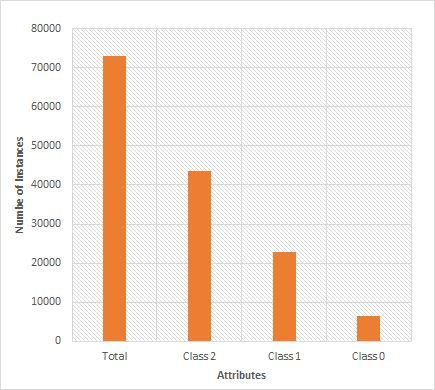
\includegraphics[width=0.4\textwidth]{class_imbalance}
	\caption{Number of instances for each class in the dataset.}
	\label{fig:class_imbalance}
\end{figure}

Class imbalance problem arises when the number of instances of one class is very large compared to the example from other class, which leads to poor accuracy of the classifier for class with less instances. Class imbalance problem can be solved using two approaches, namely data and algorithm~\cite{purwar-2014}. One popular data-based approach using clustering is called SMOTE, which has proven to be very useful for dealing with class imbalance problem~\cite{smote-2012}. We used this approach for our project. Modified SVM using decision threshold adaptation~\cite{wu-2003, raskutti-2004}, variation of likelihood estimation in decision trees~\cite{weiss-2003} are some of the algorithm approaches for data imbalance problem.

Figure~\ref{fig:class_imbalance} depicts the class imbalance problem with the dataset where the ratio between class 3 vs class 1 is 6.71. Class 1 examples were oversampled with a ratio of 6.71 using SMOTE technique. Class 2 instances were not oversampled as the number of instances of class 2 compared to class 1 was in a ratio of 1.9. Different Performance of the oversampled dataset and raw dataset is discussed in section 7.

\subsection{Data Imputation}

\begin{figure}[htpb]
	\centering
	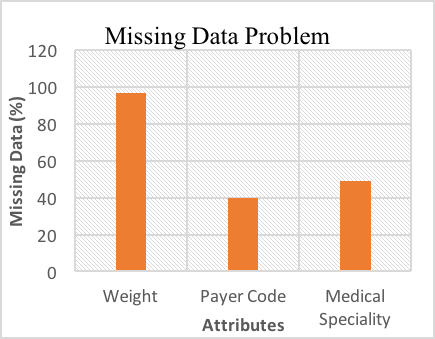
\includegraphics[width=0.4\textwidth,scale=0.7]{missing_data}
	\caption{Percentage of missing data for various features of the dataset.}
	\label{fig:missing_data}
\end{figure}

% deletion of missing data, using model-based approach to fill in values...

Missing data is a serious problem in medical databases especially with the diabetic database and that limits the use of machine learning algorithm for medical databases. However, there are various methods available to deal with the missing data problem~\cite{imputation-96}. Treatment of the missing data should be done carefully to prevent bias introduction~\cite{gustavo-2003}. Two different methods of data imputation were experimented in this project namely data deletion and data substitution using model based approach. Different model based approach such as Auto Class C4.5~\cite{lakshminarayan-1999}, k-nearest neighbour~\cite{gustavo-2003} etc. were also used for data imputation. Figure~\ref{fig:missing_data} represents the missing data in the dataset with three features having the highest percentage of missing data.

Missing data problem was dealt using two different methods i.e. Deletion Method and Model Based Substitution Method. Deletion method was applied to weight and payer code attribute while deletion and model based substitution method was utilized for medical speciality attribute. Decision tree classifier and k-nearest neighbour was used as model for substitution method as was suggested from the literature of missing data problem. Cross Validation was used for hyper parameter optimization. Target attribute was medical speciality with 70 classes and 30891 instances. Decision tree classifier performance was best with accuracy of 51.2 \% with 11 as the depth of tree. Dataset after imputation was having 72936 instances and 44 attributes and 1 target task.


\section{Performance Measurement Criteria}
% f1 score, problems with that...

\begin{figure}[htpb]
	\centering
	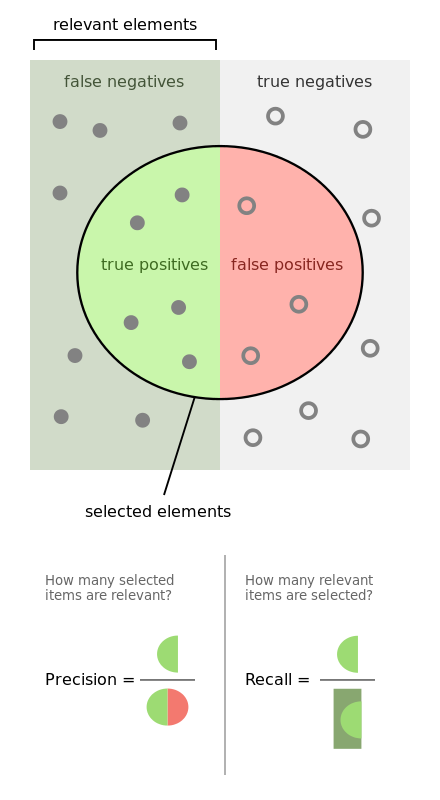
\includegraphics[width=0.5\textwidth,scale=0.5]{precision_recall}
	\caption{Pictorial representation of precision \& recall.}
	\label{fig:precision_recall}
\end{figure}

Precision was used as the performance measurement criteria for the classifiers as shown in Figure~\ref{fig:precision_recall}. Since the dataset is imbalance thus measuring the accuracy of the classifier was not a feasible criterion. Also the cost associated with classifying a patient which was readmitted as not readmitted is higher than other way around. Precision is given by the following equation.

\[ Precision = \frac{True Positive}{True Positive + False Positive} \]

\section{Methodology}

Methodologies such as Naïve Bayes, Decision Trees etc. were implemented as the baseline learner as mentioned in section 6.1 from scikit learn library. Support Vector Machines, Neural Network and Adaboost classifier was also implemented as mentioned in section 6.2, 6.3 and 6.4 respectively from scikit learn library. Dataset containing 72936 instances and 44 attributes was divided into training and testing set as 70\% / 30\%. All the results mentioned in section 7 was achieved on the testing set of 21880 instances, 44 attributes and the performance criteria used for measuring the performance of classifier was precision as mentioned in section 5. Hyper parameter associated with different classifiers were optimized via cross validation using scikit learn Grid Search CV.

\subsection{Baseline learners}

Six different baseline classifiers mentioned below were implemented for measuring the performance of baseline classifiers: Gaussian Naïve Bayes, Decision Trees, Random Forest, Linear Discriminant Analysis, Quadratic Discriminant Analysis and k-Nearest Neighbour.

\subsection{Neural Networks}

\subsection{Adaboost}
Adaboost is a machine learning ensemble method that can perform exceptionally well with classifying complex datasets. In general, ensemble methods work by training a group of weak learners on a randomly selected, 'bootstrapped' subset of the training data. The ensemble learner then makes predictions by taking a linear combination of the weak learners' classifications. This type of prediction is shown below, where \[F(x)\] is the classification of the ensemble method and \[a_{i}f_{i}(x)\] is the classification of a weak learner.

\[
	F(x) = \sum_{i} a_{i}f(x)
\]

Unlike other ensemble methods, Adaboost bootstraps subsets by weighting the data points based on whether or not they've been correctly classified by other weak learners in the group. This forces the ensemble to learn the qualities of hard-to-classify data. In general this learner has very low bias and variance and tends to generalize well to test data. It has been shown to work well for classifying health care datasets similar to the one at hand~\cite{adaboost-breast-cancer}.

\subsection{Support Vector Machines (SVM)}
SVMs are well known for being very effective learners in the realm of classifying health care data. Munnangi and Chakraborty used an linear SVM to produce the best performance model for the same classification task we were approaching [cite SAS paper]. Like many learners, SVMs construct a decision boundary through a feature space, separating one class of data from another. The decision boundary is constructed by maximizing the geometric margin between the boundary and the points closest to the boundary. Because there is a sense of a best boundary, SVMs have the powerful quality of being able to associate each data point classification with a confidence score. The farther a data point is from the boundary, the more likely it is to belong to the associated class. This is very useful in a multi class setting, where the class of a data point is the most likely class predicted by a set of decision boundaries.

With the given dataset, we explored using scikit learn's SVM with several types of kernel functions: linear, polynomial, and rbf (radial basis function). Kernel functions are used by SVMs to determine the distance between two points. The proper choice of kernel function can have a significant impact on the performance of the decision boundary. We saw a 10\% accuracy difference between a linear SVM and rbf SVM.

\section{Results}

\begin{figure*}[htpb]
	\centering
	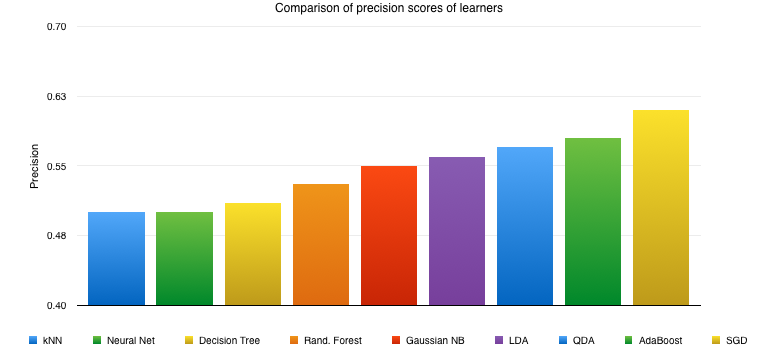
\includegraphics[width=\textwidth]{learner_comparison}
	\caption{Comparison of precision scores of learners on dataset with missing data deleted and no oversampling performed.}
	\label{fig:learner_comp}
\end{figure*}

Figure~\ref{fig:learner_comp} shows the precision scores of the various methods discussed above. Results across the board were not particularly impressive compared to the random baseline of 0.333, ranging from 0.49 to 0.61. k-Nearest Neigbor and Neural Net performed the worst. The highest-performing algorithm was the Support Vector Machine (SGD), followed by AdaBoost.

\begin{figure}[htpb]
	\centering
	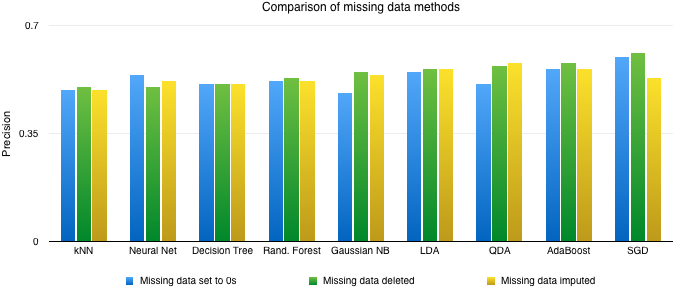
\includegraphics[width=0.5\textwidth]{missing_data_comparison}
	\caption{Comparison of missing data methods via precision scores of learners.}
	\label{fig:missing_data_comp}
\end{figure}

A comparison of the various methods to handle missing data is presented in figure~\ref{fig:missing_data_comp}, with precision scores from all learners shown. Generally, missing data set to its own category performed worse than both deletion and imputation, which each performed equally on average. There are some exceptions to this trend, specifically with Neural Networks, Gaussian Naive Bayes, and SVM, where one method is slightly better or worse than the other two.

\begin{figure}[htpb]
	\centering
	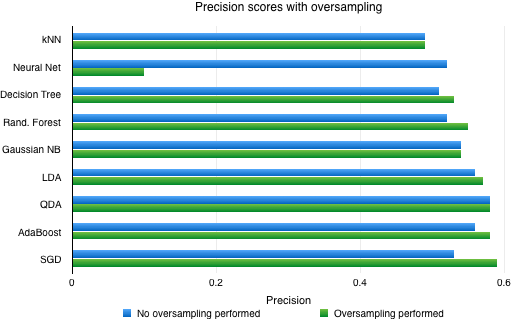
\includegraphics[width=0.5\textwidth]{oversampling_comparison}
	\caption{Precision scores of learners with and without oversampling of under-represented target classes, on a dataset with missing data deleted.}
	\label{fig:oversampling_comp}
\end{figure}

Figure~\ref{fig:oversampling_comp} shows the effect of oversampling on precision scores of the various learners. On average, oversampling of under-represented target classes performed equal to or better than not oversampling, particularly with SGD where the score improved by 0.6. One significant outlier was the Neural Network algorithm, where oversampling performed much worse than not oversampling.

\begin{figure}[htpb]
	\centering
	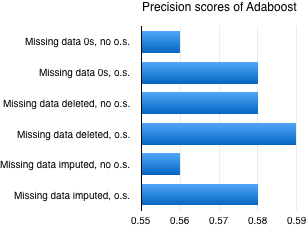
\includegraphics[width=0.5\textwidth,scale=0.75]{adaboost}
	\caption{Precision scores of Adaboost learner for various data pre-processing combinations.}
	\label{fig:adaboost}
\end{figure}

The combinations of missing data methods and oversampling are presented in figure~\ref{fig:adaboost} with precision scores using the Adaboost algorithm. Results were very similar across the combinations, with scores only ranging from 0.56 to 0.59. Deleting missing data and oversampling performed the best at 0.59, while not performing oversampling and either imputing missing data or setting it to a separate category performed the worst at 0.56.

\begin{figure}[htpb]
	\centering
	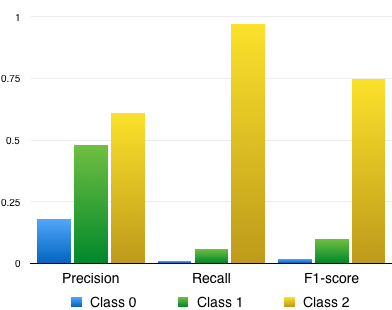
\includegraphics[width=0.5\textwidth]{full_results}
	\caption{Sample results of SGD learner on dataset with imputed missing data.}
	\label{fig:full_results}
\end{figure}

Precision, recall, and f1-score metrics for the three target classes using a sample learner (Support Vector Machines) with imputation for missing data is shown in figure~\ref{fig:full_results}. Although average values for each metric seem relatively stable (0.53 for precision, 0.60 for recall and 0.48 for f1-score), looking deeper at the breakdown of class values show an imbalance, with class 1 performing much worse than class 2, and class 2 performing much worse than class 3.

\begin{figure}[htpb]
	\centering
	\includegraphics[width=0.5\textwidth]{confmatrix_SGD_PCA}
	\caption{Confusion matrix of SGD learner with PCA on dataset with deleted missing data.}
	\label{fig:sgd_pca_results}
\end{figure}

The best results of applying PCA before SVM classification are shown below~\ref{fig:sgd_pca_results}. We found an optimal performance with keeping the 32 principal components. While the overall f1-score was significantly worse with feature selection, it did improve the precision and recall on class 0 (.41 f1-score for class 0, .35 f1-score for class 1, .46 f1-score for class 2). For each class, SVM predicted the correct class more than any other class. ANOVA produced similar but less successful results and as such the results are not shown here.

\begin{figure}[htpb]
	\centering
	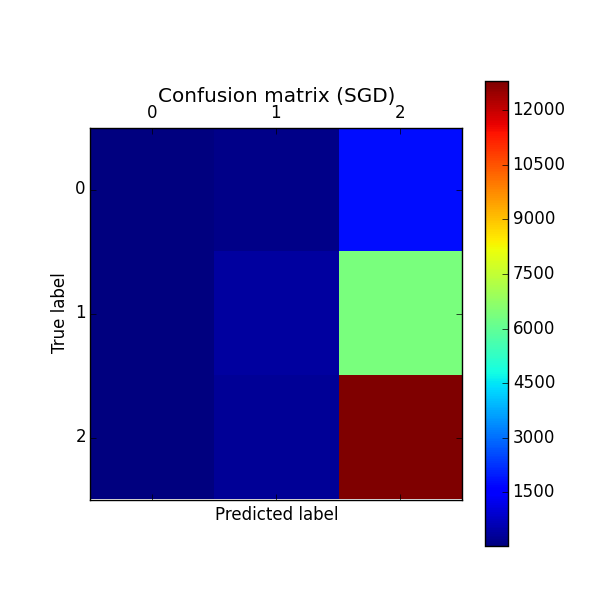
\includegraphics[width=0.25\textwidth]{full_results_confmatrix_SGD_md=imputed_ns=all_nc=3_os=f_test}
	\caption{Confusion matrix of SGD learner on dataset with imputed missing data.}
	\label{fig:full_results_cm}
\end{figure}

The confusion matrix for figure~\ref{fig:full_results} is shown in figure~\ref{fig:full_results_cm}. This figure displays that the majority of predictions are for class 2, even when the true class is 0 or 1. There are relatively much fewer predictions of class 0 or 1.

\section{Discussion}

\section{Conclusion}

\section{Future Work}


% if have a single appendix:
%\appendix[Proof of the Zonklar Equations]
% or
%\appendix  % for no appendix heading
% do not use \section anymore after \appendix, only \section*
% is possibly needed

% use appendices with more than one appendix
% then use \section to start each appendix
% you must declare a \section before using any
% \subsection or using \label (\appendices by itself
% starts a section numbered zero.)
%


\appendices
\section{Statement of Contributions}
This report is a joint contribution of all the team members. Data Imputation and Data Imbalance problem was done by Ashish. Jonathan did the algorithms for machine learning classification including neural network. Feature selection and SVM was done by Charlie.

We hereby state that all work presented in this report is that of the authors.

% references section

% can use a bibliography generated by BibTeX as a .bbl file
% BibTeX documentation can be easily obtained at:
% http://www.ctan.org/tex-archive/biblio/bibtex/contrib/doc/
% The IEEEtran BibTeX style support page is at:
% http://www.michaelshell.org/tex/ieeetran/bibtex/
%\bibliographystyle{IEEEtran}
% argument is your BibTeX string definitions and bibliography database(s)
%\bibliography{IEEEabrv,../bib/paper}
%
% <OR> manually copy in the resultant .bbl file
% set second argument of \begin to the number of references
% (used to reserve space for the reference number labels box)
%\begin{thebibliography}{1}
%\end{thebibliography}

\printbibliography

% i still have to turn these refs into bibtex...
%[2]. Lakshminarayan, Kamakshi, et al. "Imputation of Missing Data Using Machine Learning Techniques." KDD. 1996.
%[3]. Batista, Gustavo EAPA, and Maria Carolina Monard. "An analysis of four missing data treatment methods for supervised learning." Applied Artificial Intelligence 17.5-6 (2003): 519-533.
%[4]. Lakshminarayan, Kamakshi, Steven A. Harp, and Tariq Samad. "Imputation of missing data in industrial databases." Applied Intelligence 11.3 (1999): 259-275.
%[5]. Purwar, Archana, and Sandeep Kumar Singh. "Issues in data mining: A comprehensive survey." Computational Intelligence and Computing Research (ICCIC), 2014 IEEE International Conference on. IEEE, 2014.
%[6]. N. Abe, “Sampling approaches to learning from imbalanced datasets: active learning, cost sensitive learning and beyond,” ICML-KDD'2003 Workshop: Learning from Imbalanced Data Sets, 2003.
%[7]. V. López, A. Farnandez, J.M. Torres, and F. Herrera et al,” Analysis of preprocessing vs. cost-sensitive learning for imbalanced classification. Open problems on intrinsic data characteristics”, Expert Systems with Applications, vol 39, pp. 6585–6608, 2012.
%[8]. G. Wu E. Y. Chang,”Class-Boundary Alignment for Imbalanced Dataset Learning,” ICML-KDD'2003 Workshop: Learning from Imbalanced Data Sets, 2003.
%[9]. B. Raskutti and A.Kowalcyzk, “Extreme Re-balancing for SVM's: a case study,” ICML-KDD'2003 Workshop: Learning from Imbalanced Data Sets, 2003.
%[10]. G. M. Weiss and F.Provost ,” Learning when training data are costly: The effect of class distribution on tree induction,” Journal of Artificial Intelligence Research, vol. 19, pp. 315–354. October 2003.
%[13]. http://www.who.int/diabetes/action_online/basics/en/
%[18] SAS paper

% biography section
% 
% If you have an EPS/PDF photo (graphicx package needed) extra braces are
% needed around the contents of the optional argument to biography to prevent
% the LaTeX parser from getting confused when it sees the complicated
% \includegraphics command within an optional argument. (You could create
% your own custom macro containing the \includegraphics command to make things
% simpler here.)
%\begin{biography}[{\includegraphics[width=1in,height=1.25in,clip,keepaspectratio]{mshell}}]{Michael Shell}
% or if you just want to reserve a space for a photo:

\begin{IEEEbiography}[{\includegraphics[width=1in,height=1.25in,clip,keepaspectratio]{picture}}]{John Doe}
\blindtext
\end{IEEEbiography}

% You can push biographies down or up by placing
% a \vfill before or after them. The appropriate
% use of \vfill depends on what kind of text is
% on the last page and whether or not the columns
% are being equalized.

%\vfill

% Can be used to pull up biographies so that the bottom of the last one
% is flush with the other column.
%\enlargethispage{-5in}


\end{document}